\documentclass[11pt,letterpaper]{article}
\usepackage{acl2013}
\usepackage{times}
\usepackage{latexsym}
\usepackage{amsmath}
\usepackage{amssymb}
\usepackage{amsthm}
\usepackage{enumerate,enumitem}
\usepackage{verbatim}
\usepackage{mathtools}

\usepackage{graphicx}
\usepackage{algorithm}
\usepackage{algorithmic}

\DeclareMathOperator*{\argmax}{arg\,max}

%\usepackage{authordate1-4}
\usepackage{multirow}

\usepackage{color,soul}
\usepackage[usenames,dvipsnames,svgnames,table]{xcolor}
\newcommand{\Note}[1]{}
\renewcommand{\Note}[1]{\hl{[#1]}}
\newcommand{\NoteSigned}[3]{{\sethlcolor{#2}\Note{#1: #3}}}
\newcommand{\RemoveFF}[1]{\NoteSigned{Remove (FF)}{Crimson}{#1}}
\newcommand{\NoteFF}[1]{\NoteSigned{FF}{LightBlue}{#1}}
\newcommand{\NoteJE}[1]{\NoteSigned{JE}{LightGreen}{#1}}

\setlength\titlebox{6.5cm}    % Expanding the titlebox


\title{A Virtual Manipulative for Learning Log-Linear Models}


\author{
	 Author 1\\
	    XYZ Company\\
	    111 Anywhere Street\\
	    Mytown, NY 10000, USA\\
	    {\tt author1@xyz.org}
	  \And
	  Author 2\\
	    XYZ Company\\
	    111 Anywhere Street\\
	    Mytown, NY 10000, USA\\
	    {\tt author1@xyz.org}
 }
  
\date{}

\begin{document}

\maketitle

\begin{abstract}
We present a virtual manipulative for regularized conditional log-linear models. 
\end{abstract}

\section{Introduction}\label{sec:intro}
except for reading of data files, purely client-side $\Rightarrow$ very easy to set-up;
open-source;
data input format makes it extensible;
individual lessons can be tailored (e.g., hide/show buttons, different tool-tips for lessons)

Why do we focus on shapes, rather than words? \NoteFF{maybe we can argue via virtual manipulatives}

\NoteFF{what is the history of virtual manipulatives in teaching CS? NLP?} the HMM spreadsheet \cite{eisner-2002-tnlp}

\subsection{Regularized Conditional Log-Linear Models} \label{sec:model} 
\NoteFF{I'm not sure if this should be its own section, or a subsection of the introduction} 
Our aim is to provide an intuitive understanding of regularized conditional log-linear models. Given $K$ features $f_k$ representing $N$ data points $\{( x_i, y_i)\}_{i=1}^N$, we are interested in estimating distributions 
\begin{equation}
\hat{p}_{\vec{\theta}}\left(y\ \mid\ x\right) = \frac{u(x, y)}{\sum_{y'} u(x,y')},
\label{eqn:conditional_loglin}
\end{equation}
where $u(x,y)$ represents the unnormalized probability
\begin{eqnarray}
u(x,y) & = & \exp{\left(\vec{\theta}\cdot \vec{f}(x,y)\right)}\\
& = & \exp{\left(\sum_{k=1}^K \theta_k f_k(x,y)\right)}.
\end{eqnarray}
As our model $\hat{p}_{\vec{\theta}}$ is fully described by the feature weights $\vec{\theta}$, we find the weights that maximize the regularized conditional log-likelihood \eqref{eqn:reg_ll}:
\begin{equation}
F\left(\vec{\theta}\right) = \sum_{i=1}^N \log{\hat{p}_{\vec{\theta}}\left(y_i\ \mid\ x_i\right)} - C \cdot R\left(\vec{\theta}\right).
\label{eqn:reg_ll}
\end{equation}
Here, $C \ge 0$ is the regularization penalty for the regularizer $R(\vec{\theta})$. We will generally refer to the \textbf{full model} as that of \eqref{eqn:conditional_loglin} with objective \eqref{eqn:reg_ll}.

However, because the full model may present too many subtleties to be grasped all at once, we also consider ``simplified'' global models $\hat{p}_{\vec{theta}}\left(y\right)$. These context-nescient models allow students to focus initially on understanding some of the core underlying concepts of exponential models, such as feature interations and weight tradeoffs, before progressing to conditioned models.

\NoteFF{move to a later section} Using $\tilde{p}$ to represent the empirical distribution, the gradient of \eqref{eqn:reg_ll} is, in general,
\begin{equation}
\nabla_{\vec{\theta}} F = 
\mathbb{E}_{\tilde{p}}\left[\vec{f}(x,y)\right] 
- \mathbb{E}_{\hat{p}}\left[\vec{f}(x,y)\right]
- C \nabla_{\vec{\theta}}R(\vec{\theta}).
\end{equation}
We consider models where $R(\vec{\theta}) = \vec{0}$ (no regularization), $R(\vec{\theta}) = \|\vec\theta\|_1$, and $R(\vec{\theta}) = \|\vec{\theta}\|_2^2$: we special-case the optimizer to handle the non-differentiable $\ell_1$ regularization, thus providing a friendly educational environment in which the student may explore the differences between $\ell_1$ and $\ell_2$ regularization.

\section{Pedagogical Aims}
\NoteFF{Give an overview of what we want students/users to take away after completing these lessons. Note that currenlty these are simply copied from the Google doc titled ``600.465: Maxent Notes,'' with a very select number of edits here and there.}
\begin{itemize}
\item If the “striped” feature is predicted to occur less often than it actually does, you should raise its weight.
\item It’s possible to overfit the training data.  Regularization compensates for that and can in fact make you underfit.
\begin{itemize}
\item In particular, weights may zoom off to +infinity or -infinity if a feature is always or never present on the *observed* examples (may need to cook special datasets for this)
\end{itemize}
\item Interactions:
\begin{itemize} 
\item Raising one weight may reduce or reverse the need to raise other weights.  This can be seen by watching the gradient as we slide the slider.
\item Can share features across conditions and this helps regularizer even if likelihood is the same
\item Features that only fire on conditions have no effect on conditional distribution
\item Feature conjunctions: fewer vs. more features
\item Feature that everything/nothing has --- weights go to $\pm \infty$
\item Opposing features, e.g., solid vs striped, where there are only 2 options (or, red vs. blue)
\end{itemize}
\item Likelihood always goes up if you follow gradient
\begin{itemize}
\item gradient = observed - expected count (- regularizer)
\item This is evident in the LL-bar at the top
\end{itemize}
\item LL is maximized when you match the empirical (except for overfitting?)
\item Frequent conditions more influential
\item Some distributions can't be matched --- but you get generalization
\item The initial setting where all weights = 0 gives the uniform distribution.
\begin{itemize}
\item Some further understanding of the entropy view?  (See below.)
\end{itemize}
\end{itemize}

\NoteFF{Make sure to address this:} We should note that we are \textit{not} concerned with computational issues here, e.g., that of tractably computing the per-context normalization factor. While efficiently computing the normalization factor is a crucial component to practical log-linear models, our primary concern is to provide an intuitive understand. \NoteFF{work on the wording here...}

\NoteFF{It's also important to talk about convexity of the objective.} That is, we'll always find a unique $\vec{\theta^*}$ that solves \eqref{eqn:reg_ll}.

\section{Virtual Manipulative Overview}
See Figure \ref{fig:lesson1} for a screenshot.
\subsection{User Interface}
\begin{figure*}[t]
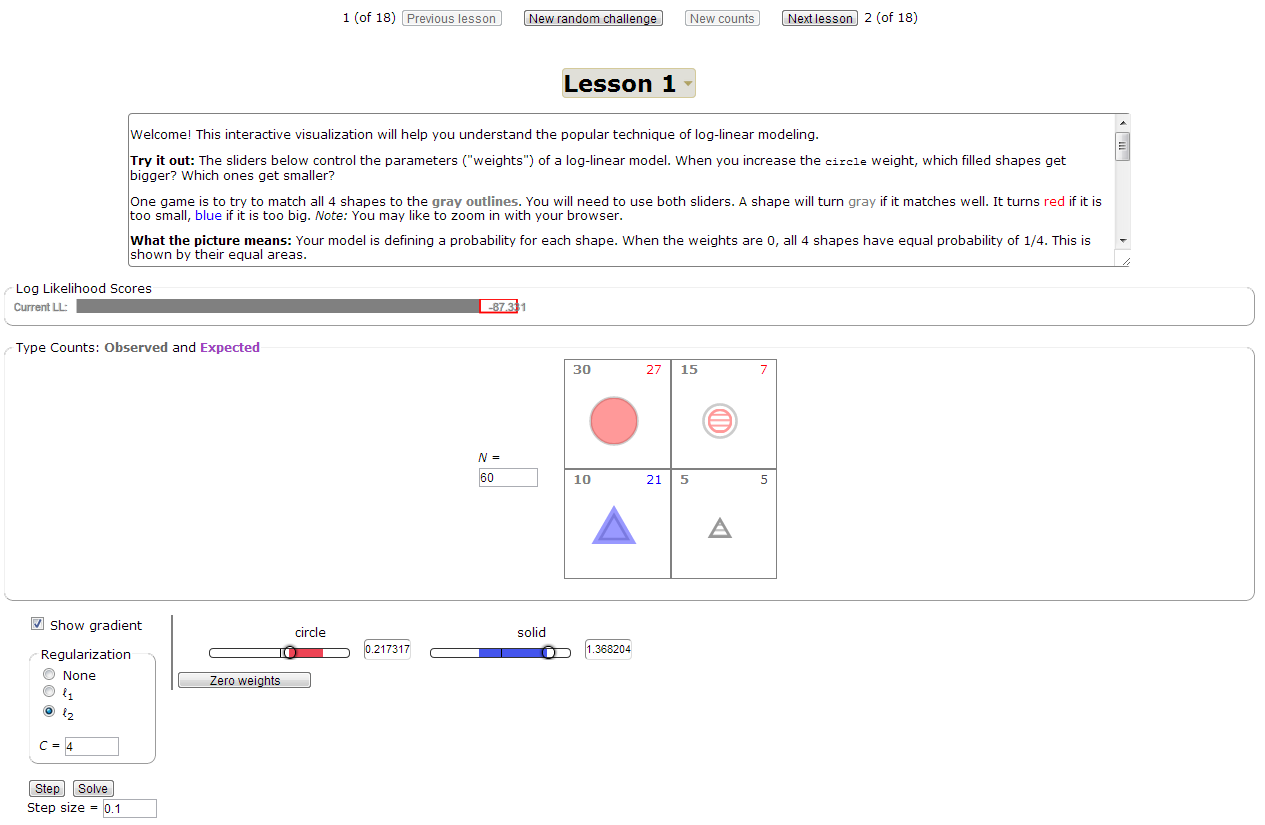
\includegraphics[scale=.5]{images/lesson1-grad-moved-nonewcounts-ell2-c4.PNG}
\caption{Screenshot of the first lesson from the virtual manipulative.}
\label{fig:lesson1}
\end{figure*}

\subsubsection{Usability}
\begin{description}
\item[``New Counts'' button] The other use is to help the user experiment with datasets of different sizes, by changing N to scale the counts and then clicking "New counts."
\end{description}

\subsection{The Instructor Interface: Creating and Tailoring Lessons}
\subsection{Data description}
\begin{description}
\item[Required]

\begin{itemize}
\item a set of contexts (if missing, will be assumed to contain only one context)
\item a set of features; some of these may be marked as hidden
\item for each context, a set of events and visual positions for them \NoteFF{explain why this visual positioning is pedagogically important, i.e., aligning \texttt{circles} vs. \texttt{triangles}, and \texttt{solid} vs. \texttt{striped} can make feature contrasts stand out more}
\end{itemize}

\item[Optional]

\begin{itemize}
\item weights for some or all features (if missing, will be imputed from the prior N(0,I) and the supplied count vectors)
If no counts are supplied, then imputation is equivalent to simple sampling from N(0,I).
More generally, imputation requires MH sampling of the feature weights (and it’s wise to initialize the sampler to a MAP estimate found by the solver).  We may not implement this case immediately, in which case the weights may stay unknown.  In that case we have to gray out a couple of buttons and treat contexts without count vectors as if they had no observations.
\end{itemize}

\item[Not done] \NoteFF{sadly, these didn't get tended to}
\begin{itemize}
\item visual positions for all visible and hidden features (if missing, will be filled in heuristically)

for each context, a total count $N_x$ (if missing, will be imputed from an integerized gamma prior and the supplied event counts and the weights)
In practice, we can forbid the lesson-maker from supplying only some of the event counts in a given context.  In that case, either the whole count vector is given and $N_x$ is just the sum, or none of the count vector is given and $N_x$ is sampled from the gamma.
for each (context, event) pair, a count (any missing counts for this context will be imputed)
In practice, we can forbid the lesson-maker from supplying only some of the event counts in a given context.  In that case, if any of this count vector is missing, then the whole thing is missing, and we can impute it simply by sampling $N_x$ events from the distribution defined by the model weights.
\end{itemize}
\end{description}

\subsection{The Back-End}
talk a bit about {\tt d3}, {\tt jQuery} and the various libraries/plugins used... nothing major, but it'll be good to outline here what exactly I used

 \section{Provided Lessons}
\begin{enumerate}
\item 
4 types: rows %%$\{triangle, circle\} X columns \{solid, striped\}$
sliders only for circle and for striped
matchable

Questions: Lead students through navigation, ask simple understanding questions. If you make striped \& circle really big, what happens to the four probabilities?  First ignore the gray outlines.  What are the probabilities and expected counts (given N) when all features are 0?  If the total score of one object is 1 or 2 more than the total score of another object, what happens to their relative probabilities?  (for example, set circle to 1 and striped to 1.  What are the relative probabilities of the 4 objects?)  What happens to the probabilities when circle goes to +infinity?  to -infinity?  What happens to the log likelihood in these cases and why?  Now try to match the gray outlines, which represent the counts you’re trying to match.  If circles overall have too low a count, you should increase circle slider: the tooltip on the slider adds up the expected and observed counts for you.  Show them the “new random challenge button.”  Encourage them to check out the tooltips.
\item same as lesson 1 but sliders for triangle, circle, solid, striped
Questions: What’s the difference between increasing triangle and decreasing circle?  What if you increase triangle and circle by the same amount?  
\item same as lesson 2 but unmatchable (“XOR problem”)
Questions: Why can’t you match the probabilities of the 4 events? This also might be a good point to ask them to work through the details of computing Z, and the individual probabilities as fractions of Z. But can you still use your four sliders to match the aggregate expected counts of the two features?  Is it enough to use just two of the sliders and leave the others at 0?  What kind of inductive bias does the model have -- i.e., how are the the probabilities being smoothed when you match those counts?    
\item same as lesson 3, but add a single conjoined feature so it’s matchable again Questions: Does it matter which conjoined feature is added?  Would it be ok to get rid of triangle and solid as in lesson 1?
\item rows {triangle, square, pentagon} x columns {solid, striped}
No features for specific shapes, but have a non-binary feature for number of sides: fires 3 times on triangle, 4 on square, 5 on pentagon.  Increasing this feature’s weight blows up pentagon at expense of triangle and perhaps expense of square.  Also have features for solid and for striped.
Question: what happens if you make the feature weight negative?  What would be different if if the feature were redefined from \# of sides to \# of sides - 3, or \# sides - 4?  If you added a pentagon feature, what would that allow you to do?
\item rows {triangle, circle, square} X columns {solid, striped, hollow}
Questions: Is it hard to match by hand?  Learn about gradient display.
\item Like lesson 6, but now unmatchable (maybe because the true model has some extra features not shown).  
Question: Learn about solver.  What solution does the model find?
\item Like lesson 7, and now the solver overfits because all of the squares have count 0: so the weight goes to -infinity and we estimate the probabilities of the squares as 0, which is not good for a smoothing method.  Learn about regularization.  Question: What effect does regularization have on the expected counts of the stripes?  How about the expected counts of the others?  On the log-likelihood? why? How is this related to smoothing?  
\item Like lesson 7, but this time get overfitting by reducing N.  Here the student should generate a number of random challenges with different values of N, and use the solver.  Question: For a given amount of regularization, is there more smoothing of the probabilities with high N or with low N?  (Distinguish between the counts and the probabilities here.)  For a given N, is there more smoothing with high or low $sigma^2$?
\item like lesson 7, but now we have too many features: we have the 9 conjoined features like triangle\&solid, triangle\&striped, etc.  So each shape can now be manipulated independently.
Question:  Note that each event now has its own feature.  This makes it easy to manipulate the probabilities individually -- try it by hand and with the solver.  The probabilities should match exactly.  Analogously, here is a fairly easy math question: Suppose you have 9 letters a,b,...i where a has feature 1 (only), b has feature 2 (only), etc.  You would like to match the observed probabilities $p(a)=p_1, p(b)=p_2$, etc., where $p_1+...+p_9=1$.  How could you set $theta_1, theta_2$, etc. to achieve this?   Because you have enough parameters to match the training data exactly, you will need some regularization for smoothing.  What is the effect of regularization in this setting where events don’t share features at all? 
\item First conditional model: brief warmup for lesson 12 below, except make them all circles and label the rows that were formerly triangle, circle, square as English, Polish, Martian (and change the feature names accordingly).  This is formally identical to lesson 12.  So we are predicting fill color based on language.  Note that we have a larger corpus of English than of Polish, and no corpus of Martian (yet!).
\item Conditional model: like lesson 7 except we now condition on the row.  “We are now showing each language as a separate shape.  Or equivalently, imagine that you already had a shape, and the event is that someone came along and picked a pattern to fill it with.  We are no longer predicting probabilities of different shapes.”  The only sliders are for solid, striped, and hollow (this is a little simpler than lesson 7).  Drop the square row for simplicity -- no, on second thought, just make that row completely unobserved so that we see generalization.  Separate the rows into different panels.  The triangle counts are (70,20,10) while the circle counts are (5,5,5) and the square counts are (0,0,0).   Note that a separate N will be shown for each context (and changing that N will generate a new random challenge in that context).  Because we have no features that pay attention to context, it’s as if we were aggregating down the column.  
Questions: What happens to triangle fit when you match the circles by hand?  How about vice-versa?  Which has the better log-likelihood and why?  If you follow the gradients to maximize the likelihood, does that fit the triangles or the circles or somewhere in between?  [The circles counts should be high enough so that the answer is clearly “in between.”]   Do the squares (unobserved) then act more like the triangles or the circles?
\item Like lesson 12, but now we have only the solid triangle (with count 100) -- so there’s only one outcome for triangles.  (The others essentially have probabilities tied to 0.)  Now the parameters only affect circles, so it pays to match the circles.  Let’s remove the hollow square as well, just for fun.
\item Like lesson 12, but add sliders for the triangle, circle, and square features (in addition to the existing solid, striped, and hollow).  Question: Why don’t these new sliders do anything?
\item Like lesson 14, but add 3 sliders for conjoined features “solid circle,” “solid triangle,” “solid square.”  These are our first bigram features, whereas solid was our unigram feature.  Question: Demonstrate multiple solutions that give you the same likelihood.  (For example, run solver from different starting points.)  Which has the best regularization penalty?   (Turn on regularization and solve again.)  How about if we use l1 regularization?  What is the effect of that on smoothing?  How is this related to backoff?  [Note: Focus this on tuning solid circle / solid triangle / solid square versus just tuning solid.  Probably the data should be generated from a model where the backoff features like solid are indeed strong.  Also, make $sigma^2$ large so that the regularization penalty is easier to see.]
\item Logistic regression.  Contexts are the following phrases or objects being classified:
…
...
In each context we have a hollow circle for “no” and a solid circle for “yes”.  (Might be better to show as  - and +.)  The features are always features of the context conjoined with blue:
solid\&...
solid\&...
Maybe classify languages as Indo-European or agglutinative or something?  But classifying baby names as male vs. female is probably better.  The observed counts are the number of times that name has been observed attached to a boy vs. a girl.  Pick a small set of names to use as data.  We can have features for multisyllabic, \# of syllables (this is integer-valued), starts with a vowel, ends with a vowel, ends with -a, ends with -ja, and prevalence in sports (this is a real number in [0,1], perhaps the fraction of days that it appears in the sports section of the newspaper).  “Venus” might be misclassified.  Emphasize that many more features could be generated manually or automatically (link to nltk lesson).
\item Multi-class regression.  Here the outputs are 3 parts of speech or something.  The features might be the word and the preceding word.  
\end{enumerate}

\bibliography{tnlp}
\bibliographystyle{acl}

\end{document}
